\chapter{Resultados detallados del aerofrenado por planeta}
\label{ap:aero-planetas}

En el capítulo de resultados (sección~\ref{sec:res-ia-aero}) el comportamiento del agente
de aerofrenado se ilustró con un cuerpo representativo (Marte) y con figuras de resumen que
abarcan los siete cuerpos con atmósfera. Este apéndice recoge, por completitud, las
figuras individuales de cada planeta: la comparación del agente con la estrategia ingenua
y la circularización de la órbita. Todas corresponden al escenario de referencia y se han
obtenido ejecutando los agentes entrenados.

% ---------------------------------------------------------------------------
\section{Agente frente a estrategia ingenua}
\label{ap:aero-tonta}

Para cada cuerpo se compara el agente de aprendizaje por refuerzo con una estrategia
ingenua que mantiene el perigeo en un valor alto y fijo. En todos los casos el agente
baja el perigeo y completa la maniobra en muchas menos  (figuras~\ref{fig:ap-tonta-venus} a~\ref{fig:ap-tonta-neptuno}).

\begin{figure}[htbp]
  \centering
  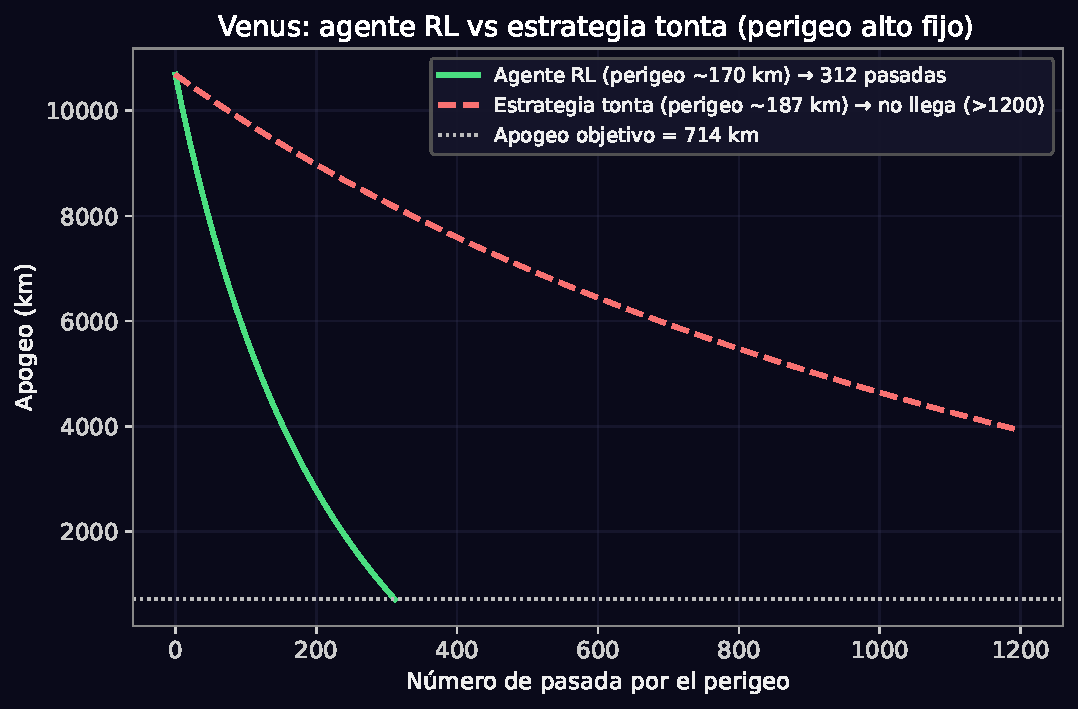
\includegraphics[width=0.78\textwidth]{tex/imagenes/ia_aero_vs_tonta_venus.pdf}
  \caption{Aerofrenado en Venus: agente frente a estrategia ingenua.}
  \label{fig:ap-tonta-venus}
\end{figure}

\begin{figure}[htbp]
  \centering
  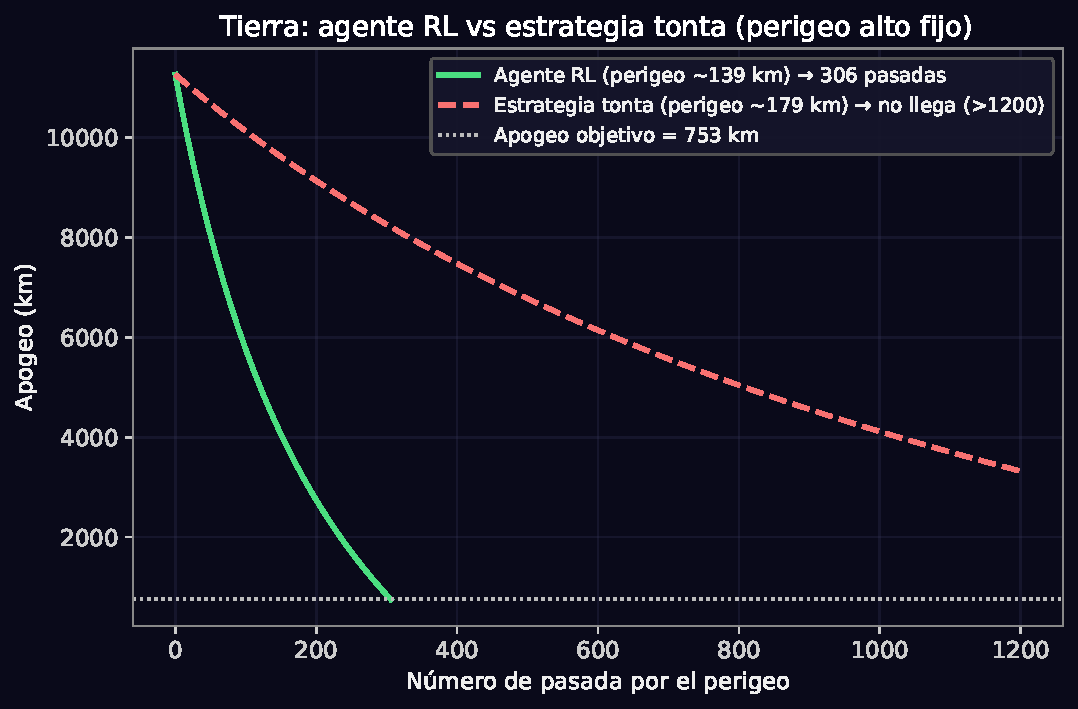
\includegraphics[width=0.78\textwidth]{tex/imagenes/ia_aero_vs_tonta_tierra.pdf}
  \caption{Aerofrenado en la Tierra: agente frente a estrategia ingenua.}
  \label{fig:ap-tonta-tierra}
\end{figure}

\begin{figure}[htbp]
  \centering
  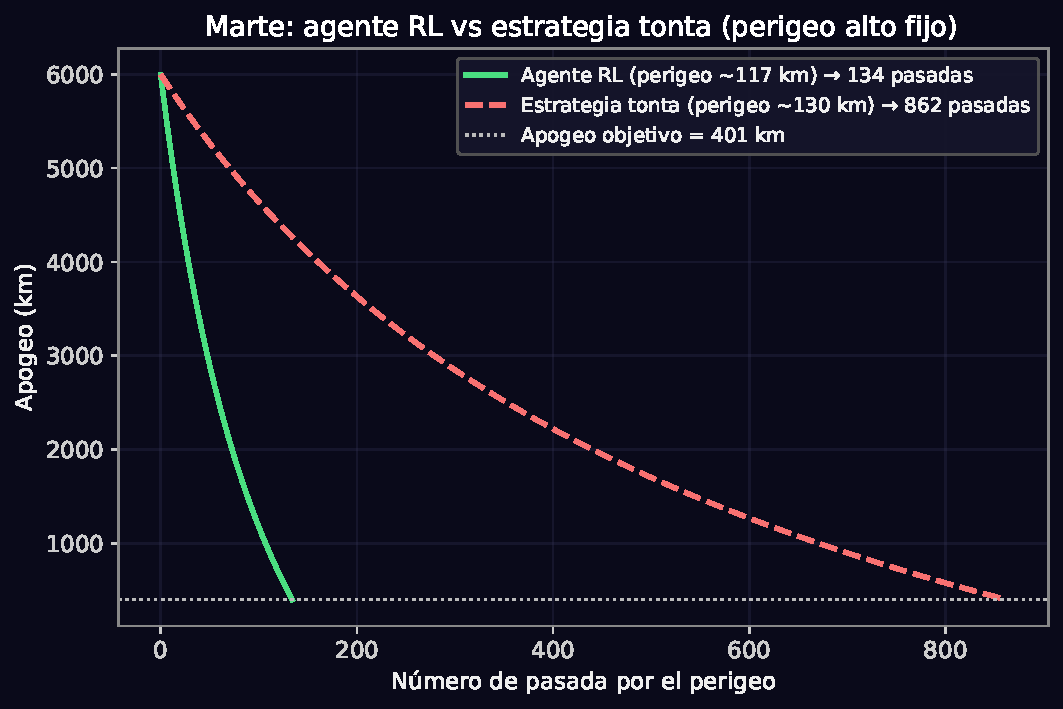
\includegraphics[width=0.78\textwidth]{tex/imagenes/ia_aero_vs_tonta_marte.pdf}
  \caption{Aerofrenado en Marte: agente frente a estrategia ingenua.}
  \label{fig:ap-tonta-marte}
\end{figure}

\clearpage

\begin{figure}[htbp]
  \centering
  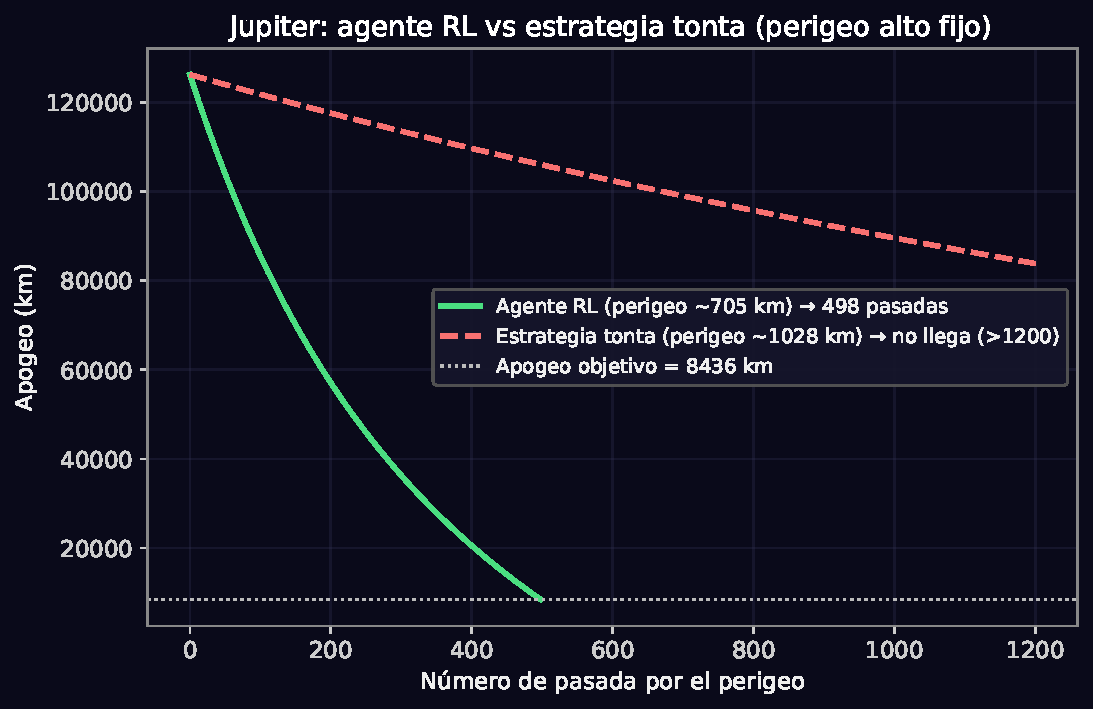
\includegraphics[width=0.78\textwidth]{tex/imagenes/ia_aero_vs_tonta_jupiter.pdf}
  \caption{Aerofrenado en Júpiter: agente frente a estrategia ingenua.}
  \label{fig:ap-tonta-jupiter}
\end{figure}

\begin{figure}[htbp]
  \centering
  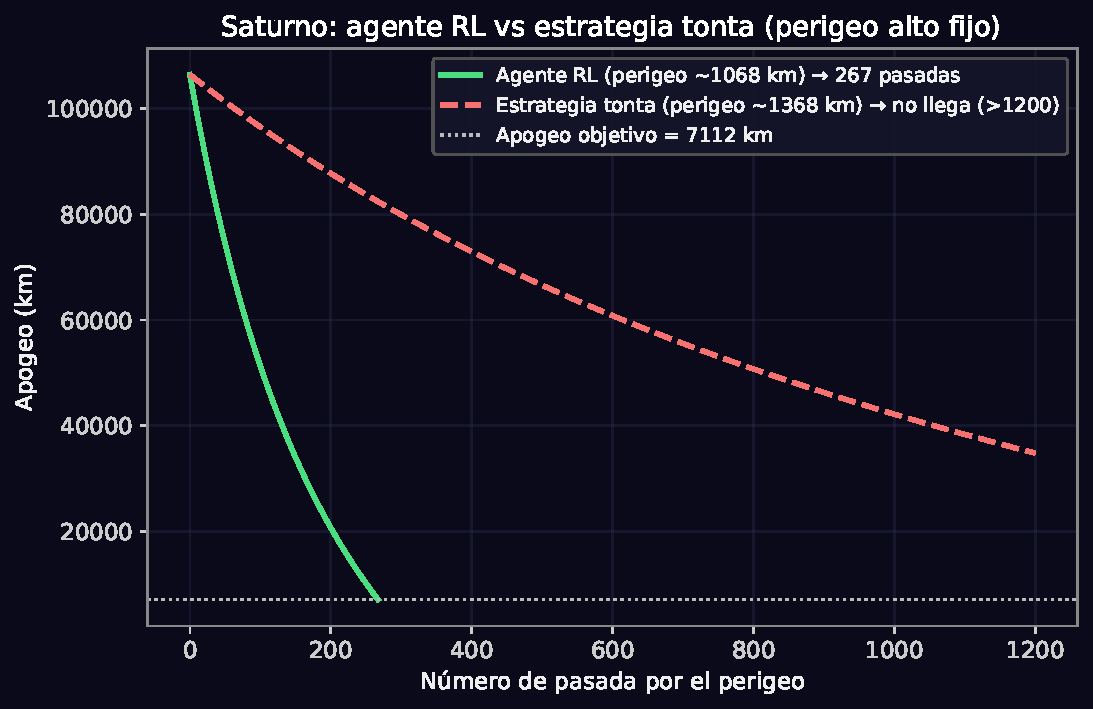
\includegraphics[width=0.78\textwidth]{tex/imagenes/ia_aero_vs_tonta_saturno.pdf}
  \caption{Aerofrenado en Saturno: agente frente a estrategia ingenua.}
  \label{fig:ap-tonta-saturno}
\end{figure}

\begin{figure}[htbp]
  \centering
  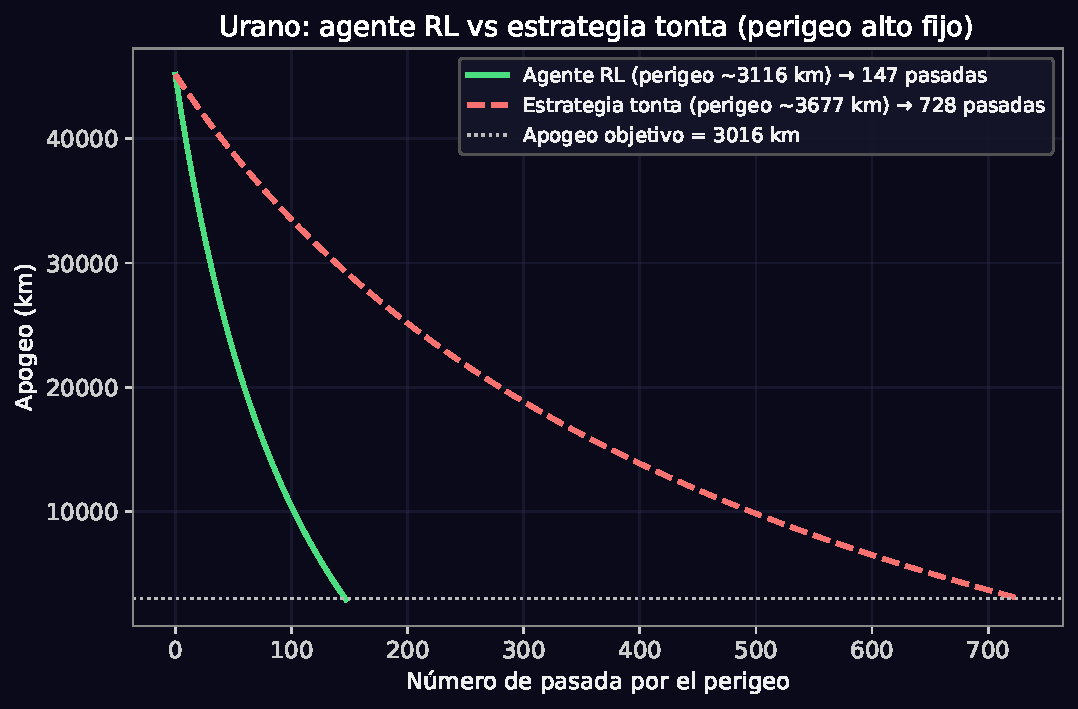
\includegraphics[width=0.78\textwidth]{tex/imagenes/ia_aero_vs_tonta_urano.pdf}
  \caption{Aerofrenado en Urano: agente frente a estrategia ingenua.}
  \label{fig:ap-tonta-urano}
\end{figure}

\clearpage

\begin{figure}[htbp]
  \centering
  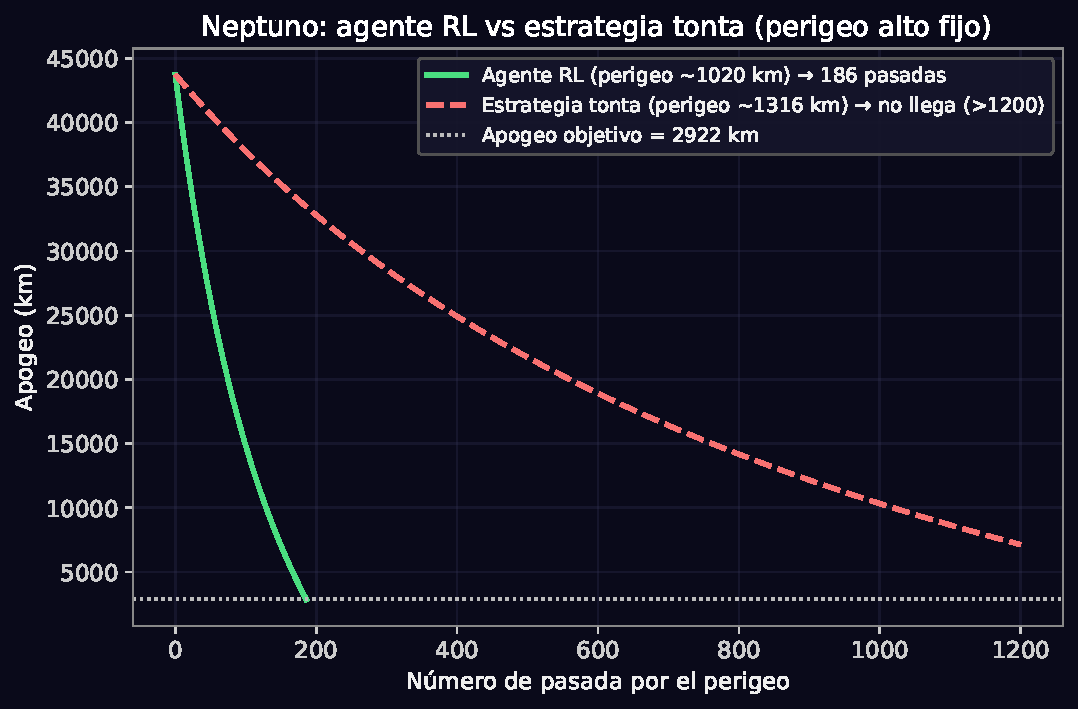
\includegraphics[width=0.78\textwidth]{tex/imagenes/ia_aero_vs_tonta_neptuno.pdf}
  \caption{Aerofrenado en Neptuno: agente frente a estrategia ingenua.}
  \label{fig:ap-tonta-neptuno}
\end{figure}

\clearpage

% ---------------------------------------------------------------------------
\section{Circularización de la órbita}
\label{ap:aero-orbita}

Para cada cuerpo se representa, en el plano orbital, cómo la órbita pasa de muy elíptica a
prácticamente circular a lo largo del aerofrenado. El cuerpo se sitúa en el centro y cada
elipse es una de las sucesivas órbitas, de apogeo decreciente (figuras~\ref{fig:ap-orbita-venus} a~\ref{fig:ap-orbita-neptuno}).

\begin{figure}[htbp]
  \centering
  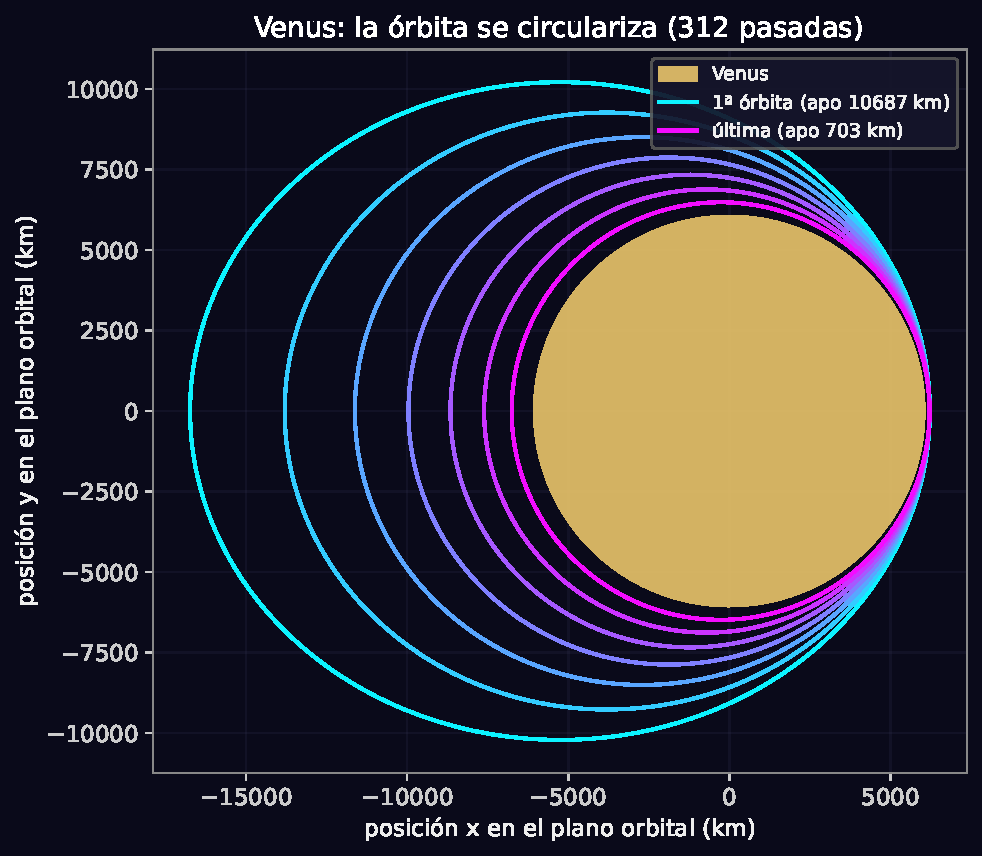
\includegraphics[width=0.55\textwidth]{tex/imagenes/ia_aero_orbita_venus.pdf}
  \caption{Circularización de la órbita por aerofrenado en Venus.}
  \label{fig:ap-orbita-venus}
\end{figure}

\begin{figure}[htbp]
  \centering
  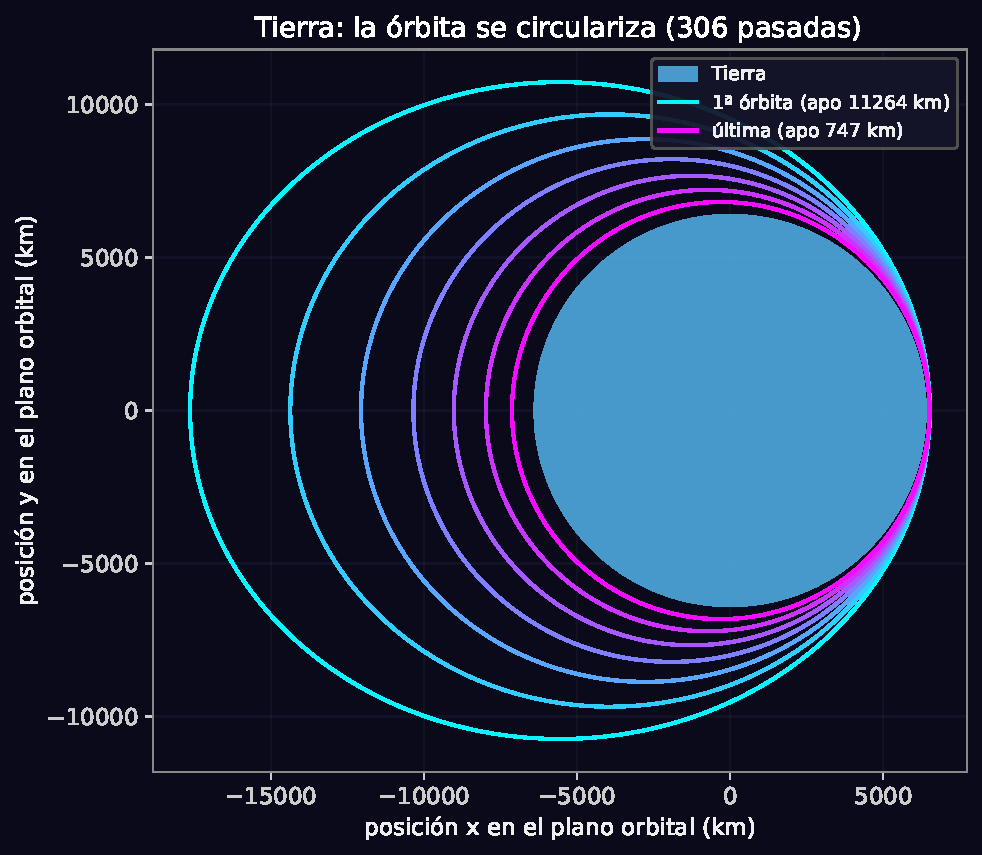
\includegraphics[width=0.55\textwidth]{tex/imagenes/ia_aero_orbita_tierra.pdf}
  \caption{Circularización de la órbita por aerofrenado en la Tierra.}
  \label{fig:ap-orbita-tierra}
\end{figure}

\begin{figure}[htbp]
  \centering
  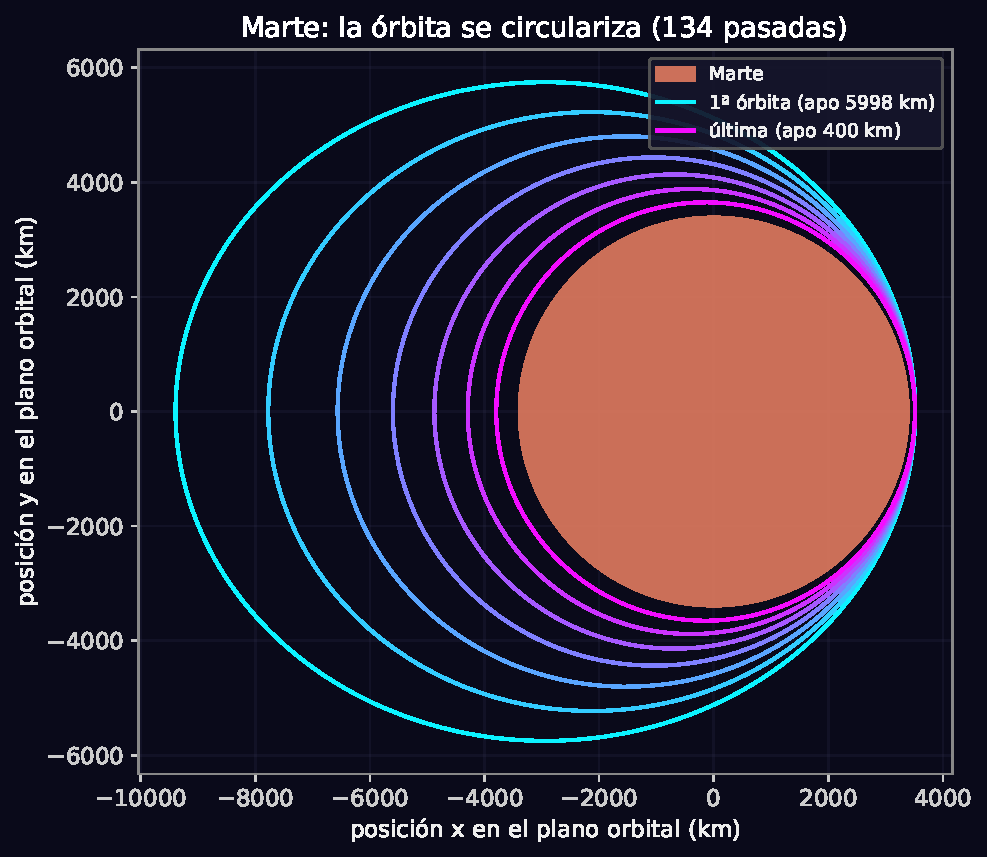
\includegraphics[width=0.55\textwidth]{tex/imagenes/ia_aero_orbita_marte.pdf}
  \caption{Circularización de la órbita por aerofrenado en Marte.}
  \label{fig:ap-orbita-marte}
\end{figure}

\clearpage

\begin{figure}[htbp]
  \centering
  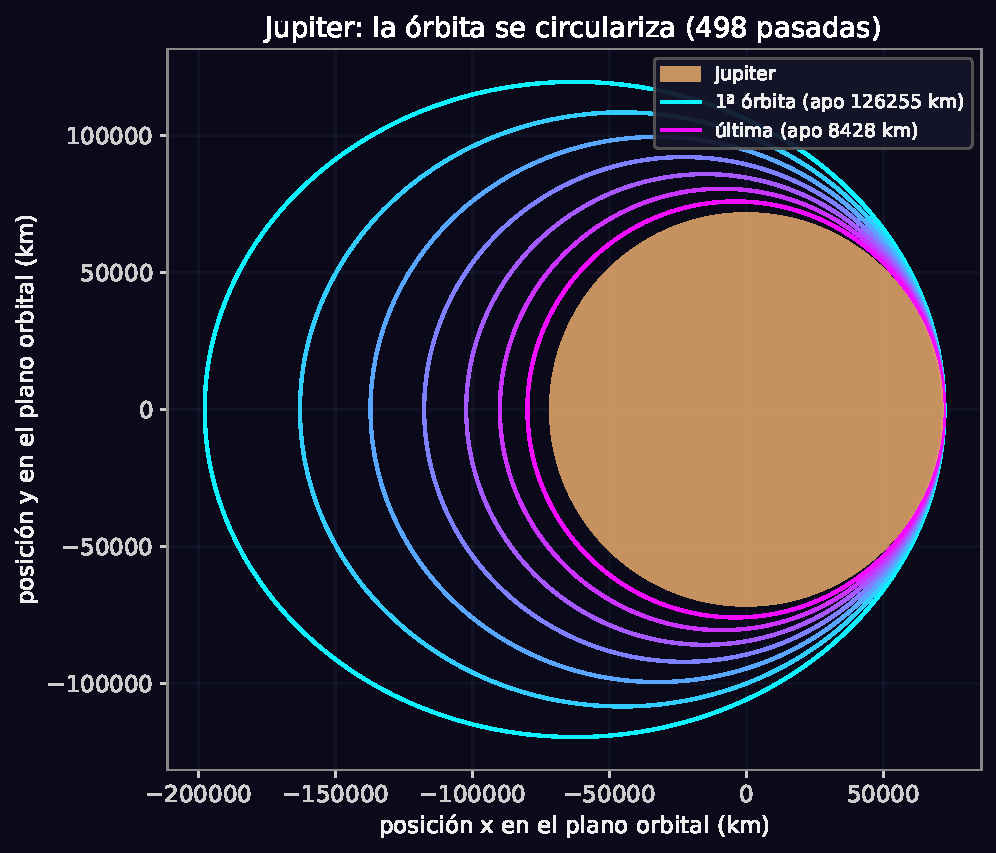
\includegraphics[width=0.55\textwidth]{tex/imagenes/ia_aero_orbita_jupiter.pdf}
  \caption{Circularización de la órbita por aerofrenado en Júpiter.}
  \label{fig:ap-orbita-jupiter}
\end{figure}

\begin{figure}[htbp]
  \centering
  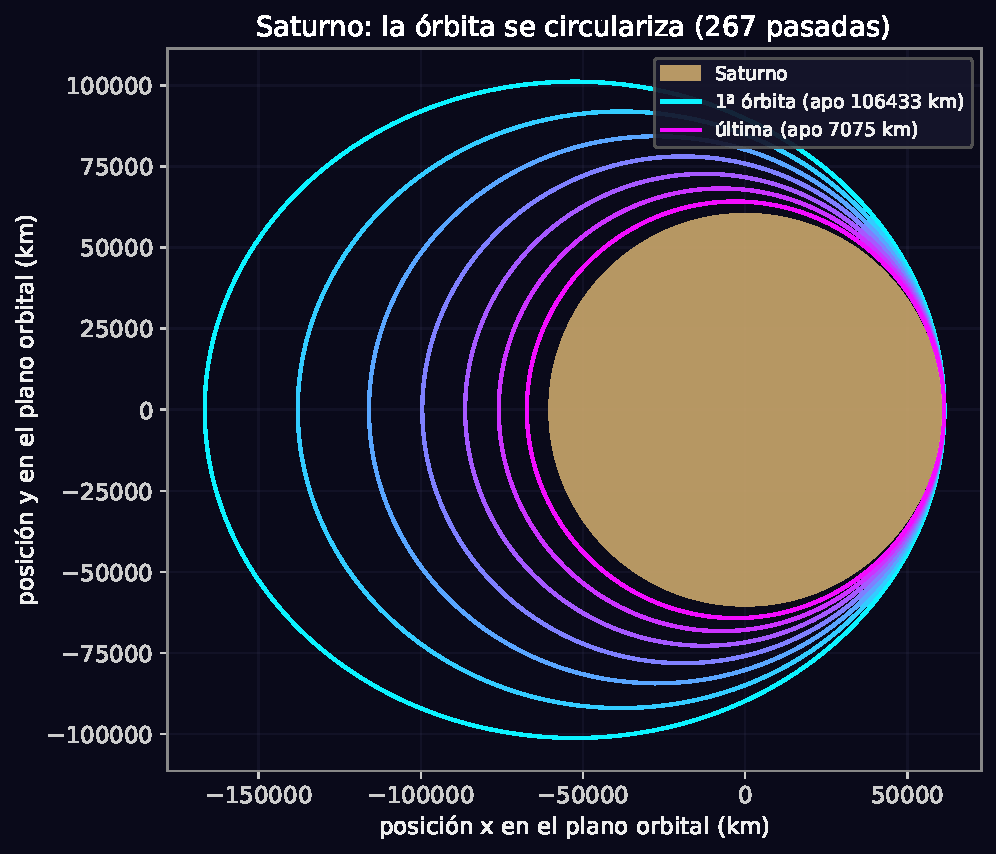
\includegraphics[width=0.55\textwidth]{tex/imagenes/ia_aero_orbita_saturno.pdf}
  \caption{Circularización de la órbita por aerofrenado en Saturno.}
  \label{fig:ap-orbita-saturno}
\end{figure}

\begin{figure}[htbp]
  \centering
  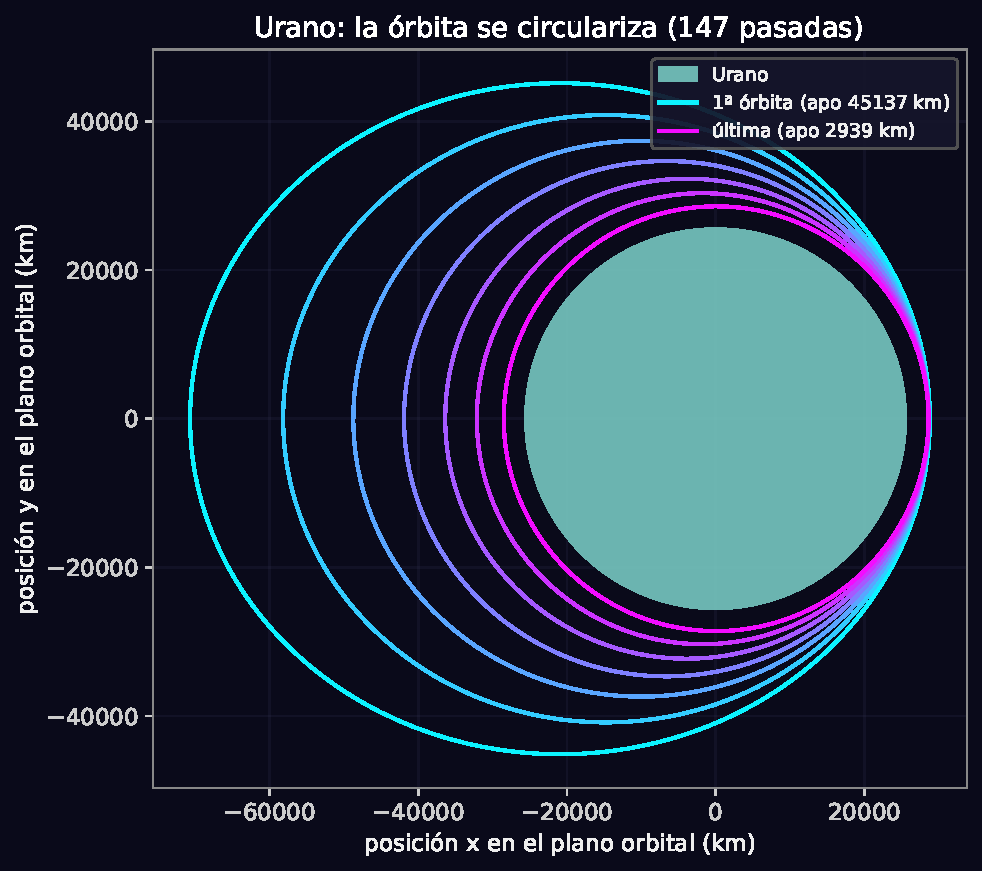
\includegraphics[width=0.55\textwidth]{tex/imagenes/ia_aero_orbita_urano.pdf}
  \caption{Circularización de la órbita por aerofrenado en Urano.}
  \label{fig:ap-orbita-urano}
\end{figure}

\clearpage

\begin{figure}[htbp]
  \centering
  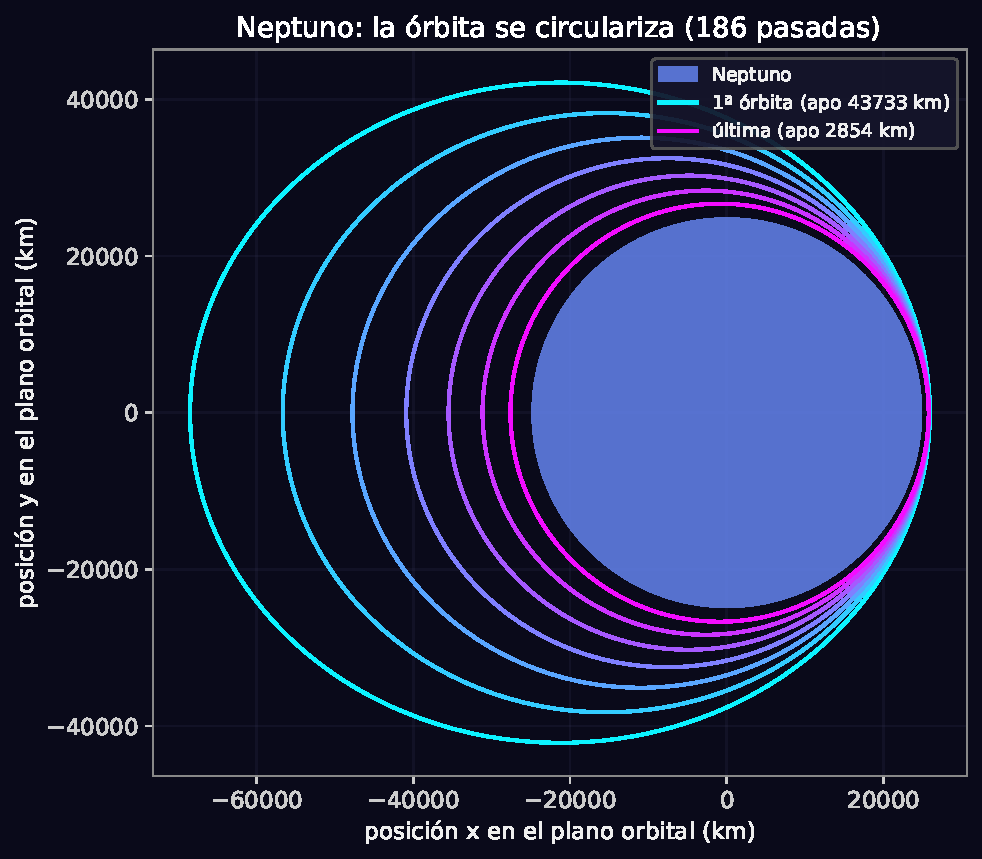
\includegraphics[width=0.55\textwidth]{tex/imagenes/ia_aero_orbita_neptuno.pdf}
  \caption{Circularización de la órbita por aerofrenado en Neptuno.}
  \label{fig:ap-orbita-neptuno}
\end{figure}
